\subsubsection{WBS} \label{sec:5-WBS}
\hypertarget{sec:5-WBS}{}
En esta sección se detalla la estructura de desglose del trabajo del proyecto también conocida como WBS, \textit{Work Breakdown Structure}. 
En ella se especifican las tareas necesarias para obtener los productos detallados en \coloredUnderline{\hyperlink{sec:5-PBS}{\ref*{sec:5-PBS} \nameref*{sec:5-PBS}}}.

Estas tareas se representan en forma de árbol jerárquico, donde cada rama representa una tarea y sus subramas las tareas que la componen.
El diagrama se ha dividido en las fases en las que se divide el proyecto para mejorar la legibilidad, facilitando la comprensión de las tareas y sub-tareas que se deben realizar en cada una de ellas.

\subsubsubsection{WBS. Visión general}
En la \coloredUnderline{\hyperlink{fig:5_WBS-Vision-General}{Figura \ref*{fig:5_WBS-Vision-General}: \nameref*{fig:5_WBS-Vision-General}}} se muestra la estructura de desglose del trabajo del proyecto de alto nivel, es decir, 
las tareas generales o fases que se deben realizar para cumplir con los objetivos del proyecto.
En las siguientes secciones, se entrará en detalle en cada una de las tareas.
\begin{figure}[H]
    \hypertarget{fig:5_WBS-Vision-General}{}
    \centering
    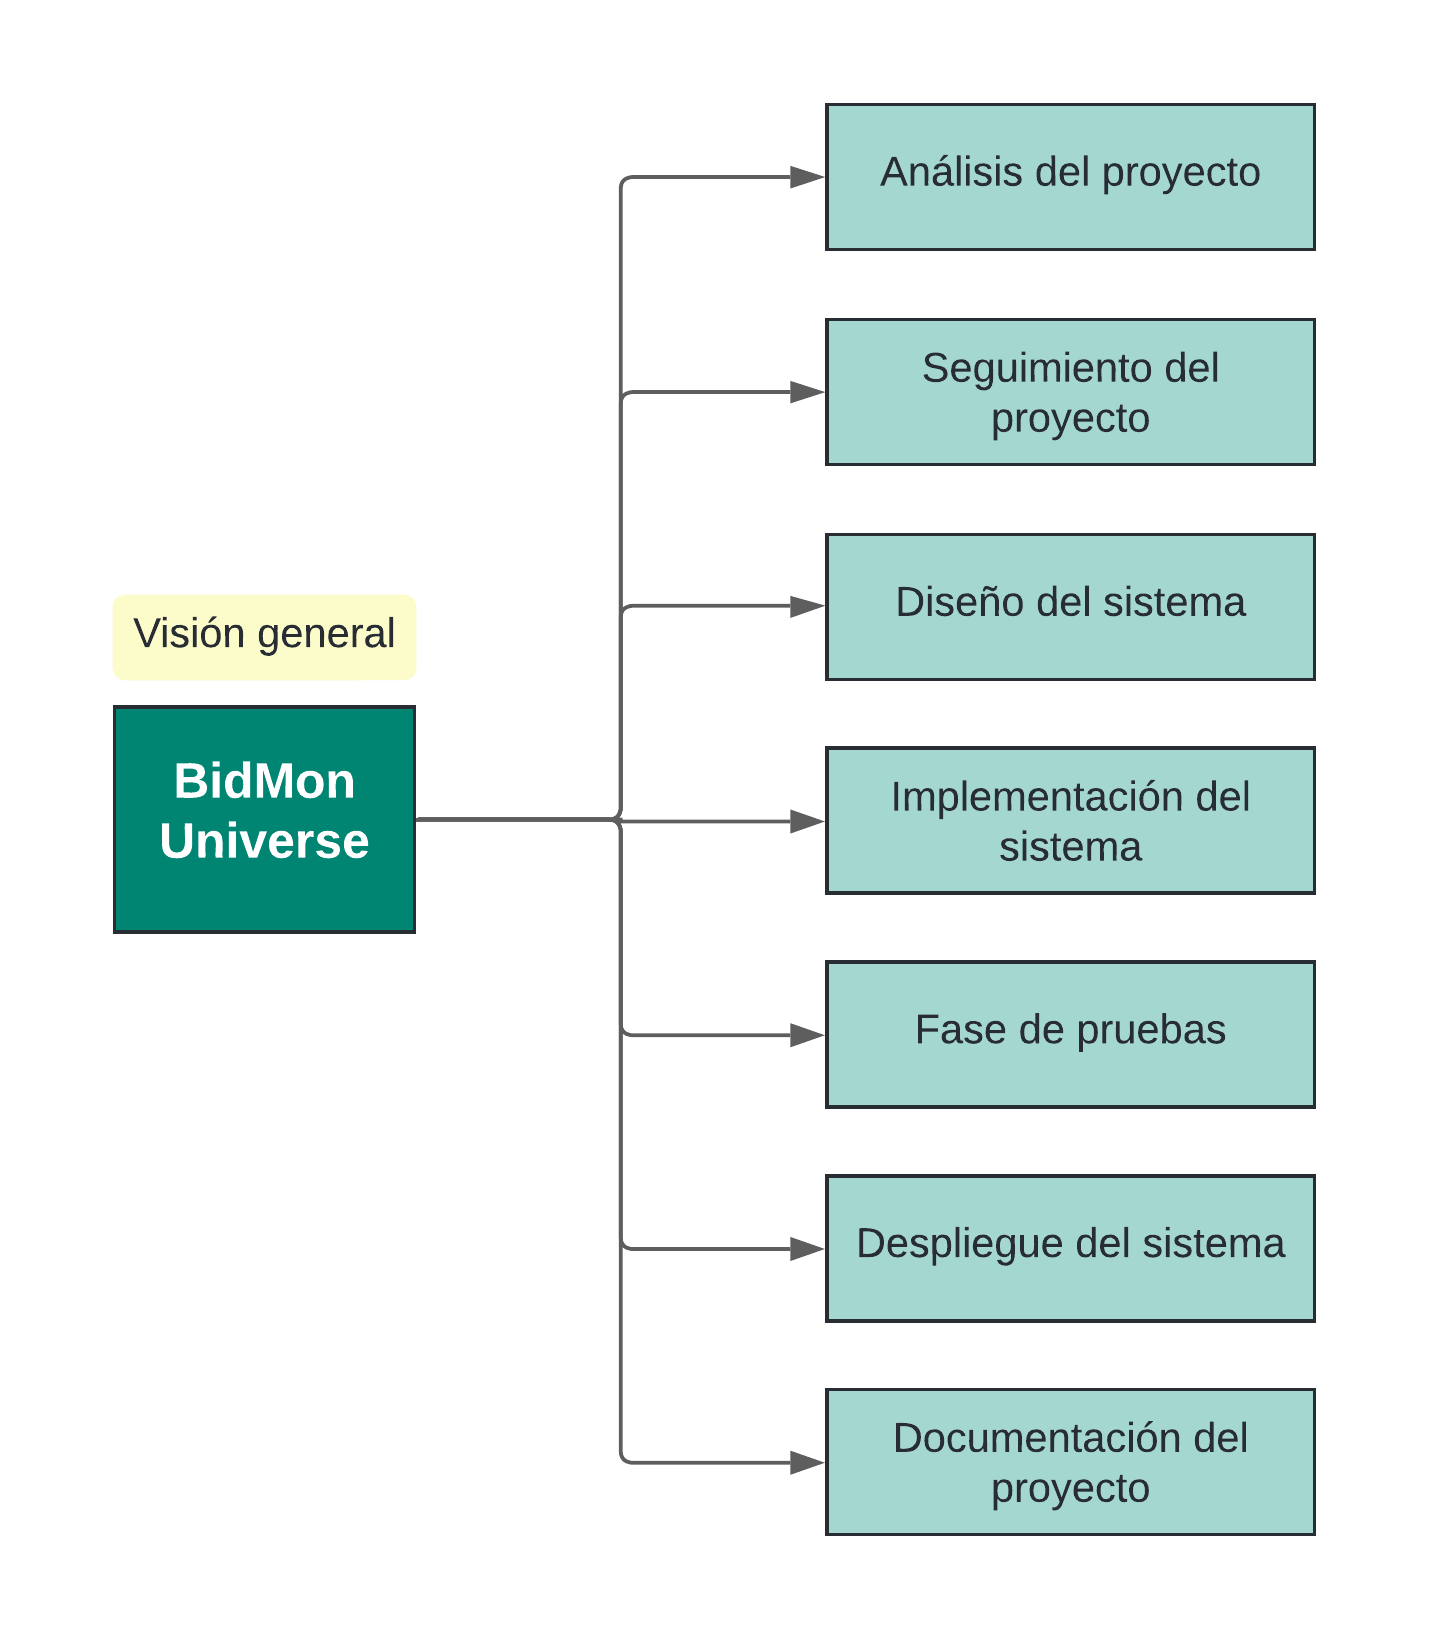
\includegraphics[width=0.5\linewidth]{figures/5-WBS/5_WBS-Vision-General.png}
    \caption{WBS. Visión general}
    \label{fig:5_WBS-Vision-General}
\end{figure}

\subsubsubsection{WBS. Análisis del proyecto}
En la \coloredUnderline{\hyperlink{fig:5_WBS-Analisis}{Figura \ref*{fig:5_WBS-Analisis}: \nameref*{fig:5_WBS-Analisis}}}, se detallan las tareas que se deben realizar en la fase de análisis del sistema para cumplir con los objetivos del proyecto.
\begin{figure}[H]
    \hypertarget{fig:5_WBS-Analisis}{}
    \centering
    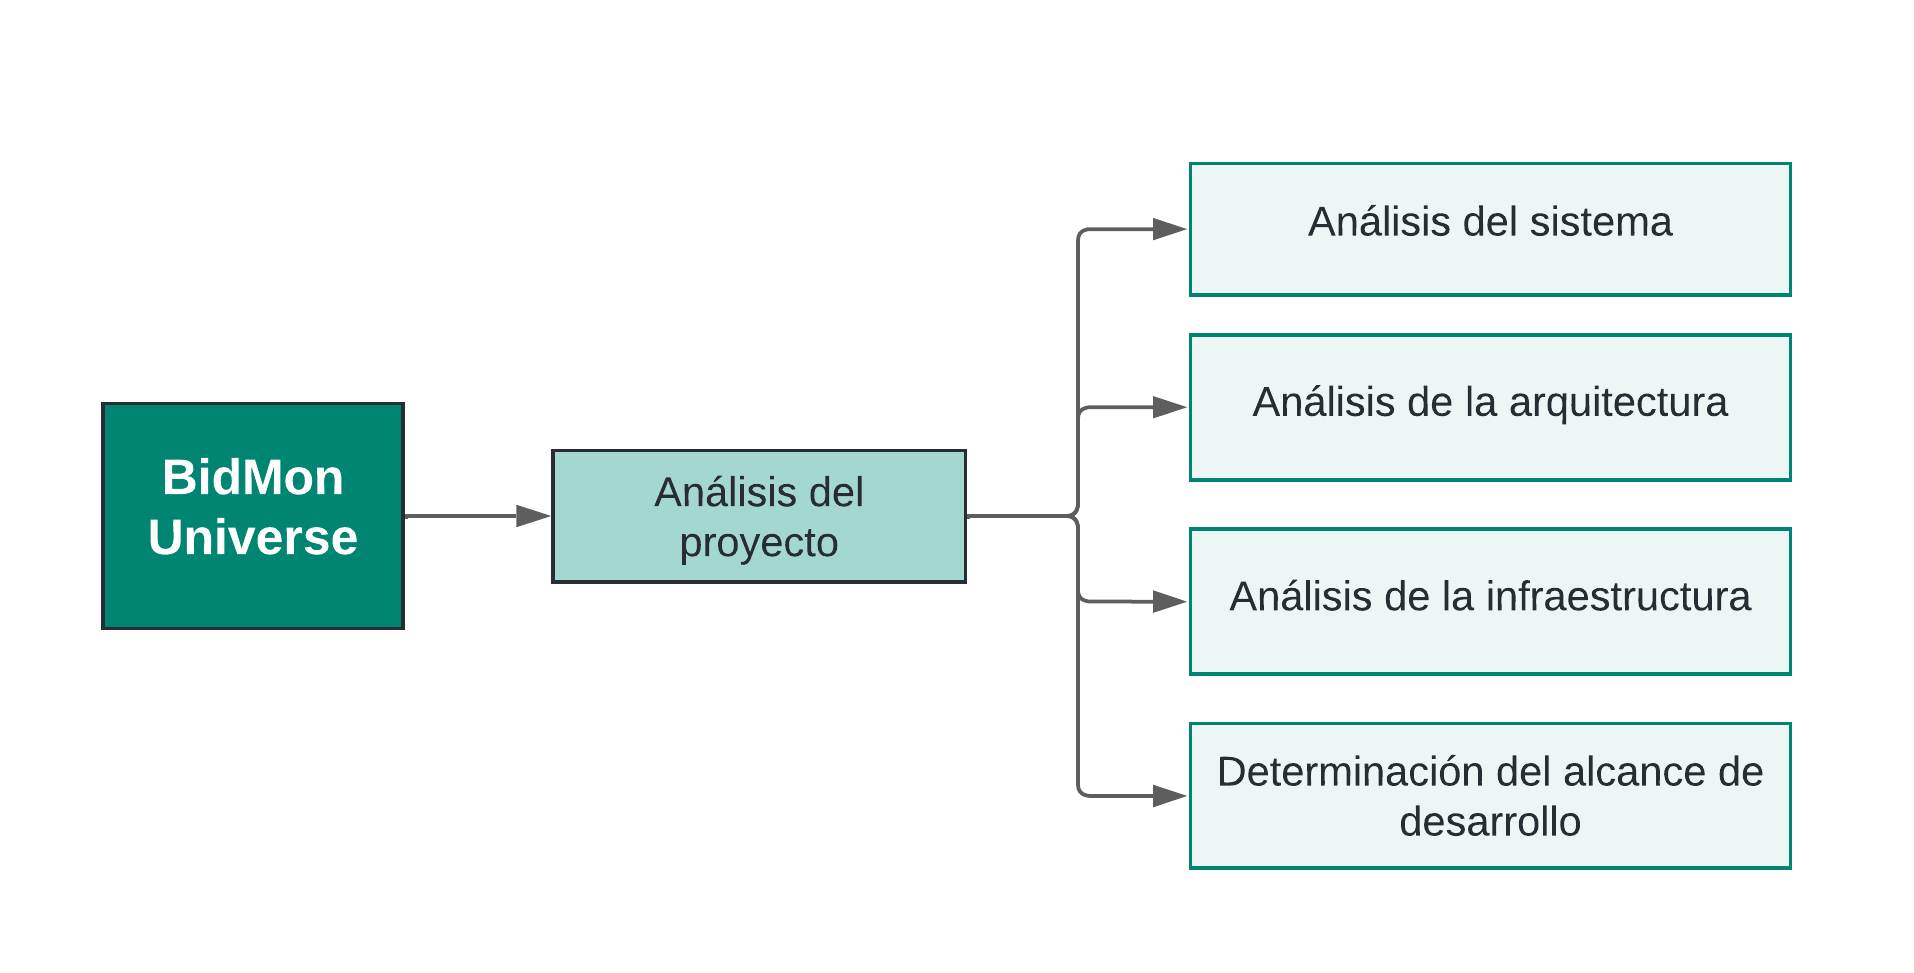
\includegraphics[width=0.7\linewidth]{figures/5-WBS/5_WBS-Analisis.png}
    \caption{WBS. Análisis del proyecto}
    \label{fig:5_WBS-Analisis}
\end{figure}

\subsubsubsection{WBS. Seguimiento del sistema}
En esta fase se realizan las tareas de seguimiento del proyecto, a través de distintas reuniones en las que se recopilará infomarción sobre el avance del proyecto. 
\begin{figure}[H]
    \hypertarget{fig:5_WBS-Seguimiento}{}
    \centering
    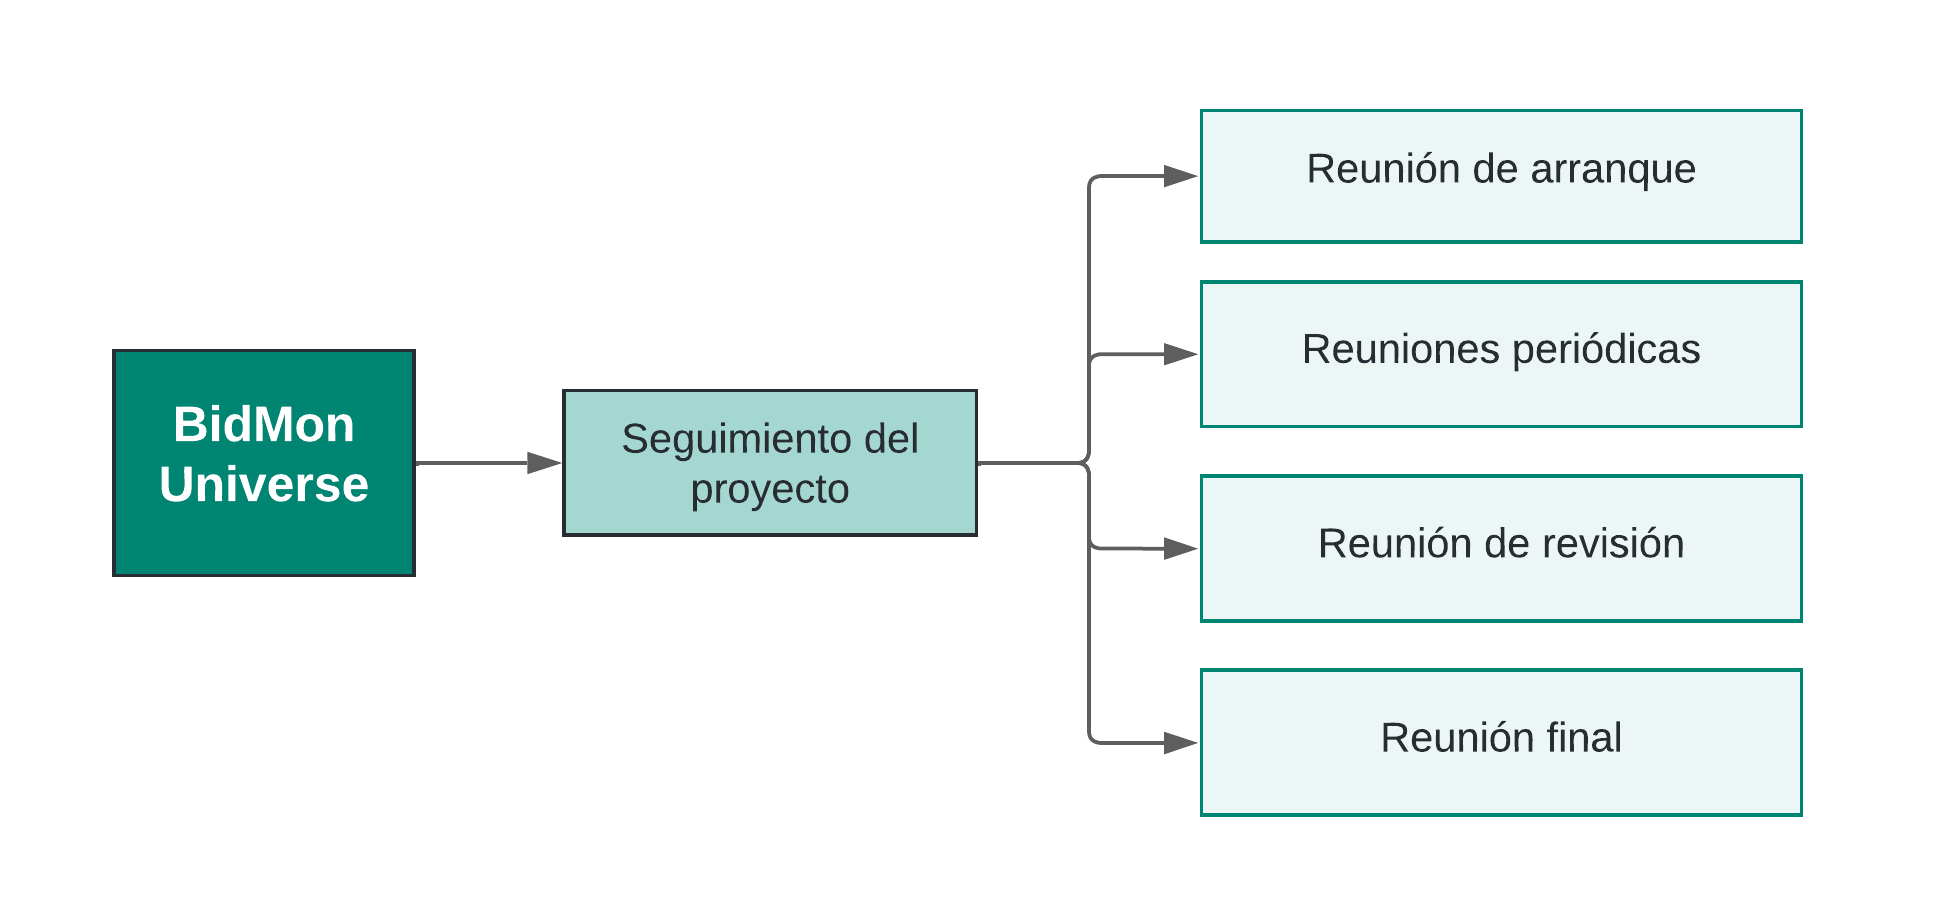
\includegraphics[width=0.7\linewidth]{figures/5-WBS/5_WBS-Seguimiento.png}
    \caption{WBS. Seguimiento del sistema}
    \label{fig:5_WBS-Seguimiento}
\end{figure}

\subsubsubsection{WBS. Diseño del sistema}
En la \coloredUnderline{\hyperlink{fig:5_WBS-Diseno}{Figura \ref*{fig:5_WBS-Diseno}: \nameref*{fig:5_WBS-Diseno}}}, se detallan las tareas que se deben realizar en la fase de diseño del sistema.
\begin{figure}[H]
    \hypertarget{fig:5_WBS-Diseno}{}
    \centering
    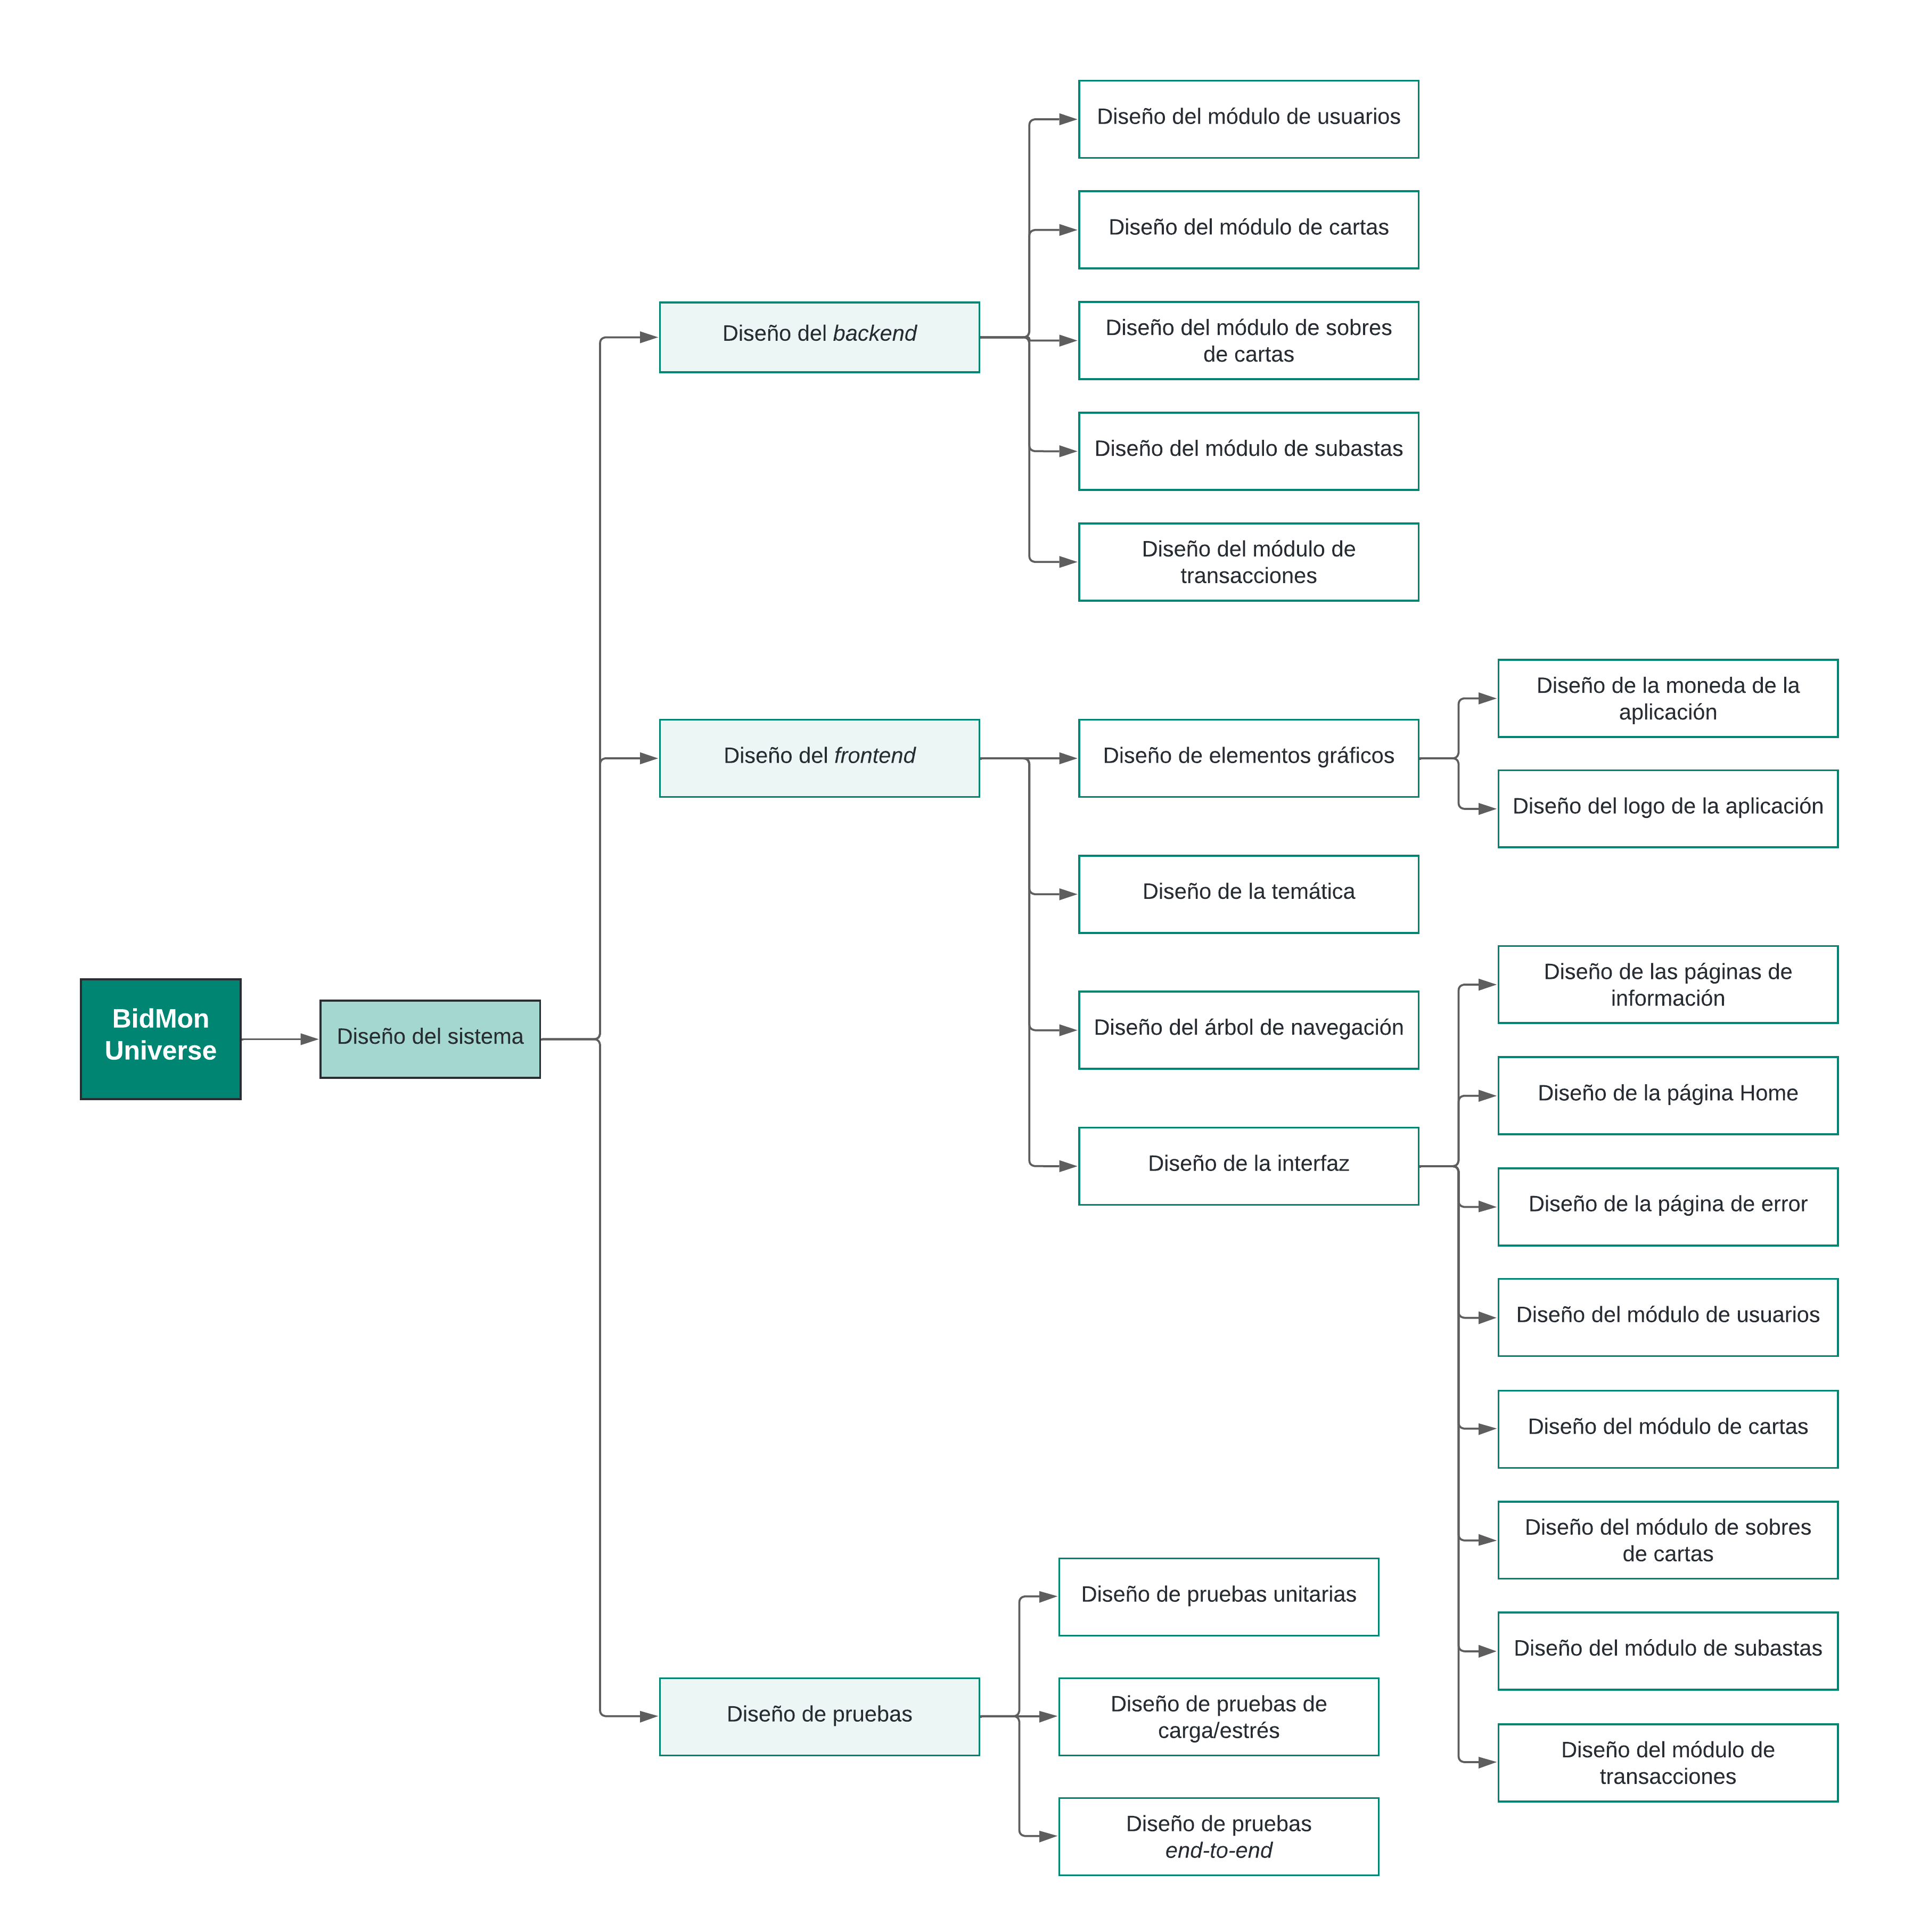
\includegraphics[width=0.9\linewidth]{figures/5-WBS/5_WBS-Diseno.png}
    \caption{WBS. Diseño del sistema}
    \label{fig:5_WBS-Diseno}
\end{figure}

\subsubsubsection{WBS. Implementación del sistema}
En la \coloredUnderline{\hyperlink{fig:5_WBS-Implementacion}{Figura \ref*{fig:5_WBS-Implementacion}: \nameref*{fig:5_WBS-Implementacion}}}, se detallan las tareas que se deben realizar en la fase de implementación del sistema.
\begin{figure}[H]
    \hypertarget{fig:5_WBS-Implementacion}{}
    \centering
    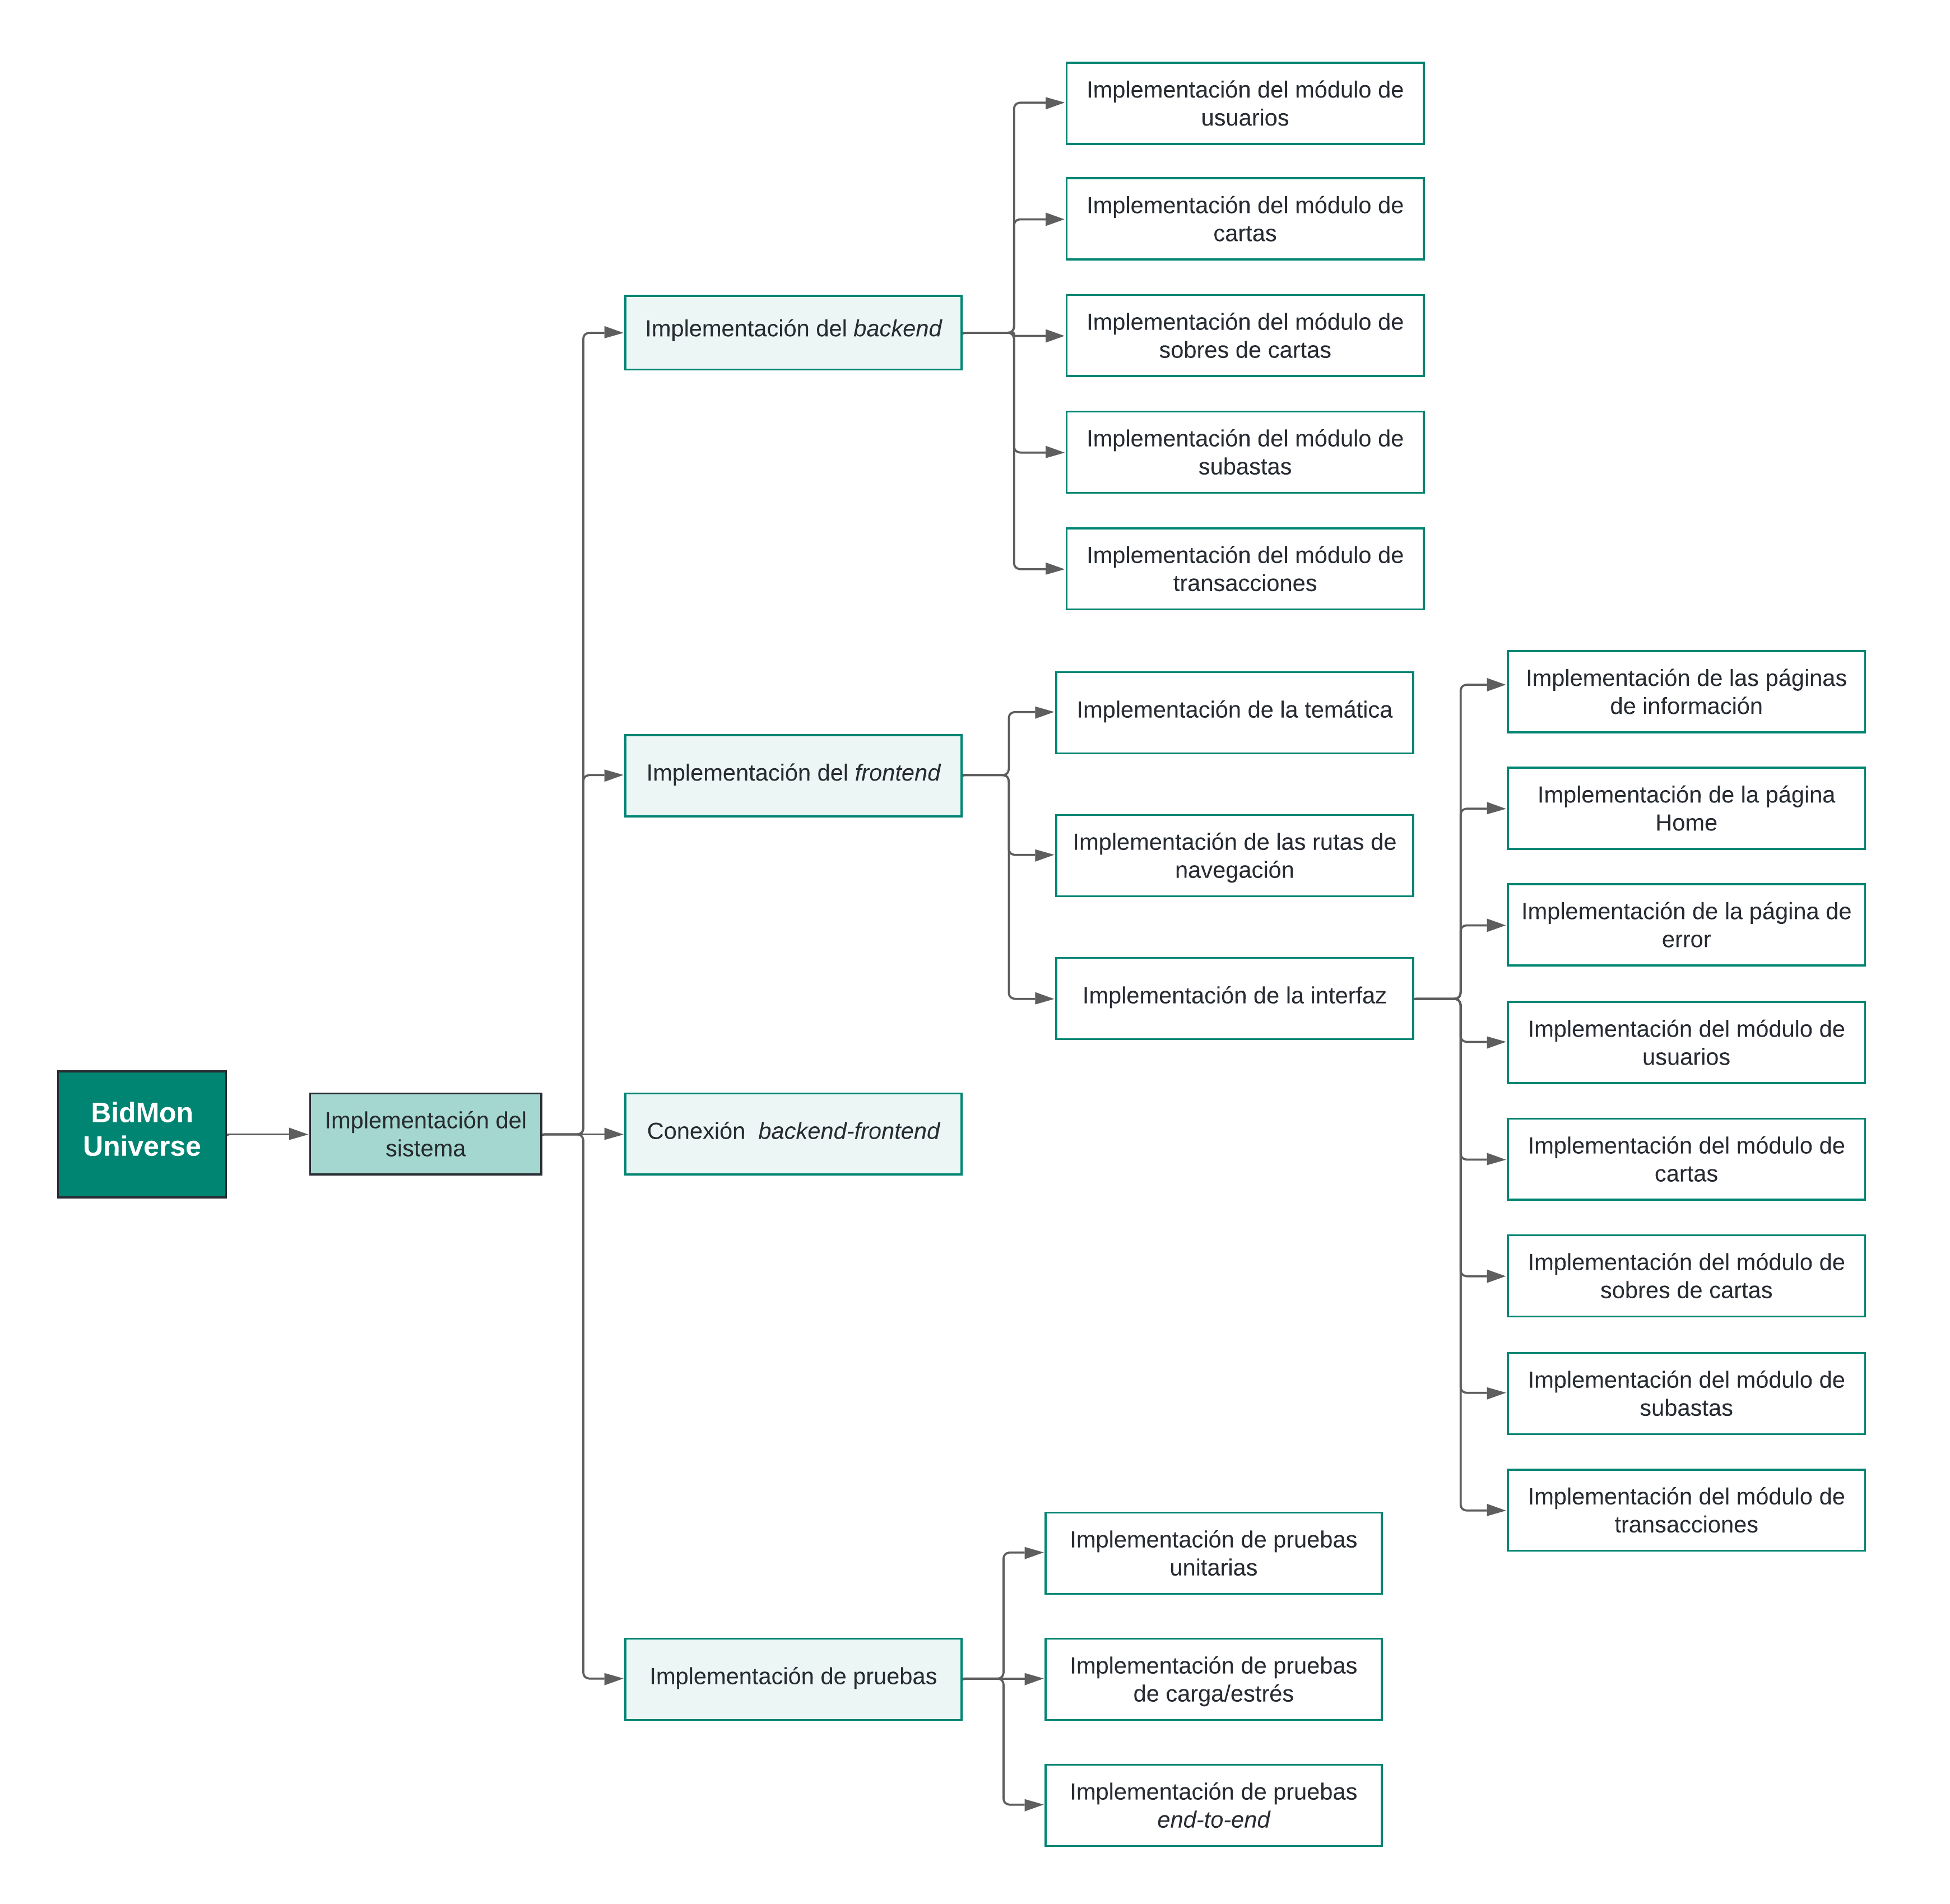
\includegraphics[width=0.9\linewidth]{figures/5-WBS/5_WBS-Implementacion.png}
    \caption{WBS. Implementación del sistema}
    \label{fig:5_WBS-Implementacion}
\end{figure}

\subsubsubsection{WBS. Fase de pruebas}
En la fase de pruebas del sistema se realizan las tareas necesarias para comprobar que el sistema cumple con los requisitos establecidos, recogiendo los informes especificados en \coloredUnderline{\hyperlink{fig:5_PBS-Pruebas}{Figura \ref*{fig:5_PBS-Pruebas}: \nameref*{fig:5_PBS-Pruebas}}}.
\begin{figure}[H]
    \hypertarget{fig:5_WBS-Pruebas}{}
    \centering
    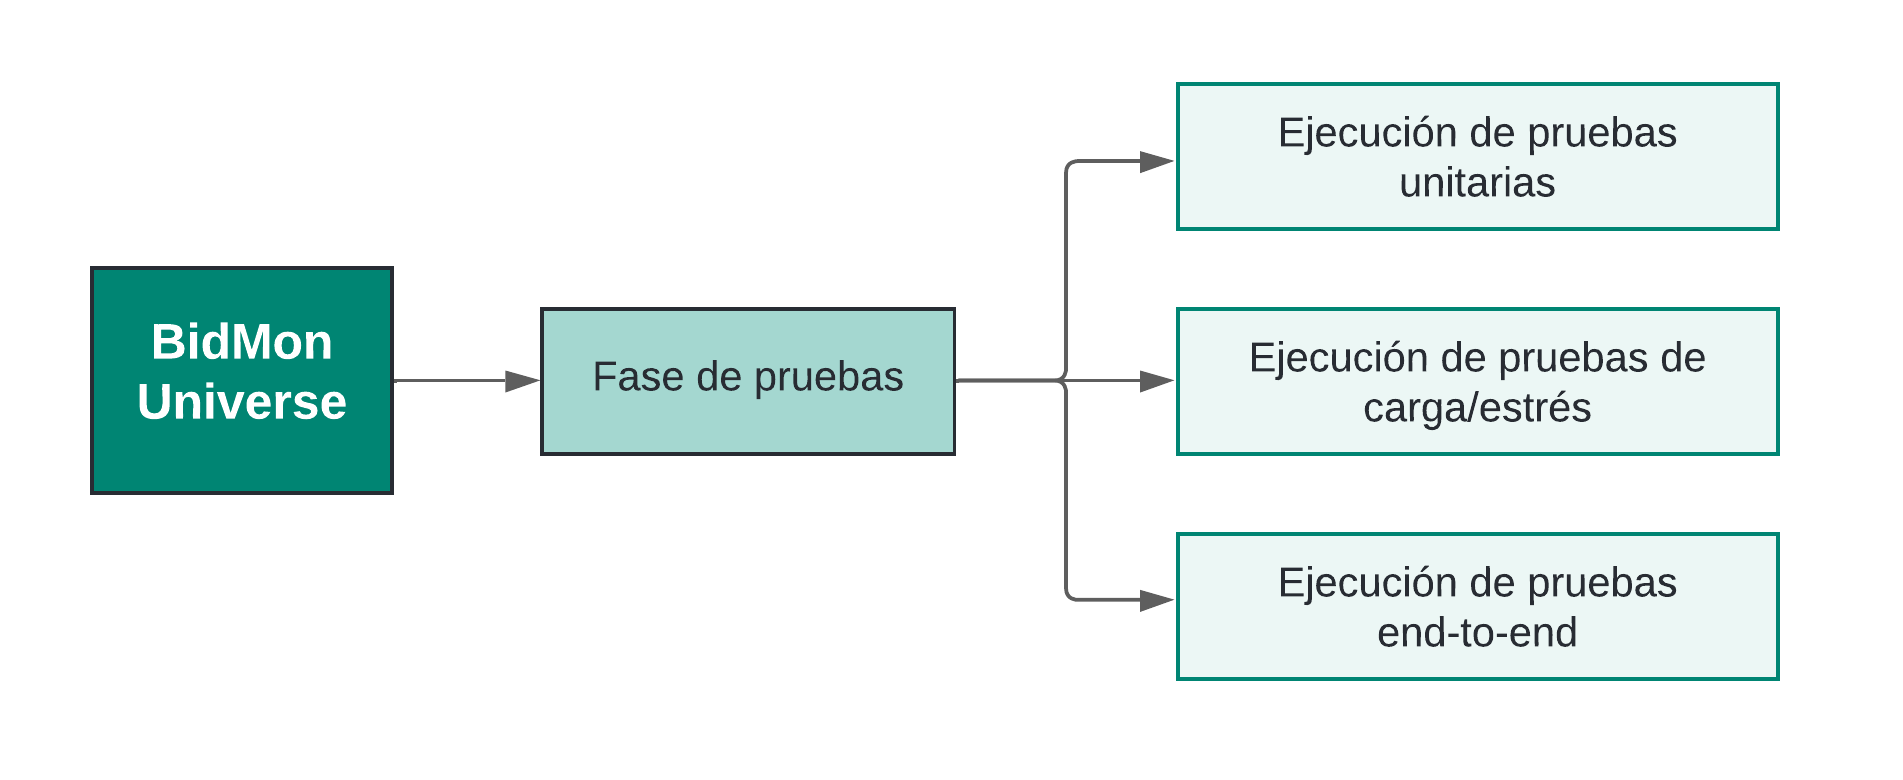
\includegraphics[width=0.9\linewidth]{figures/5-WBS/5_WBS-Pruebas.png}
    \caption{WBS. Fase de pruebas}
    \label{fig:5_WBS-Pruebas}
\end{figure}

\subsubsubsection{WBS. Despliegue del sistema}
En la fase de despliegue del sistema se realizan las tareas necesarias para poner en producción el sistema, como se detalla en la \coloredUnderline{\hyperlink{fig:5_WBS-Despliegue}{Figura \ref*{fig:5_WBS-Despliegue}: \nameref*{fig:5_WBS-Despliegue}}}.
\begin{figure}[H]
    \hypertarget{fig:5_WBS-Despliegue}{}
    \centering
    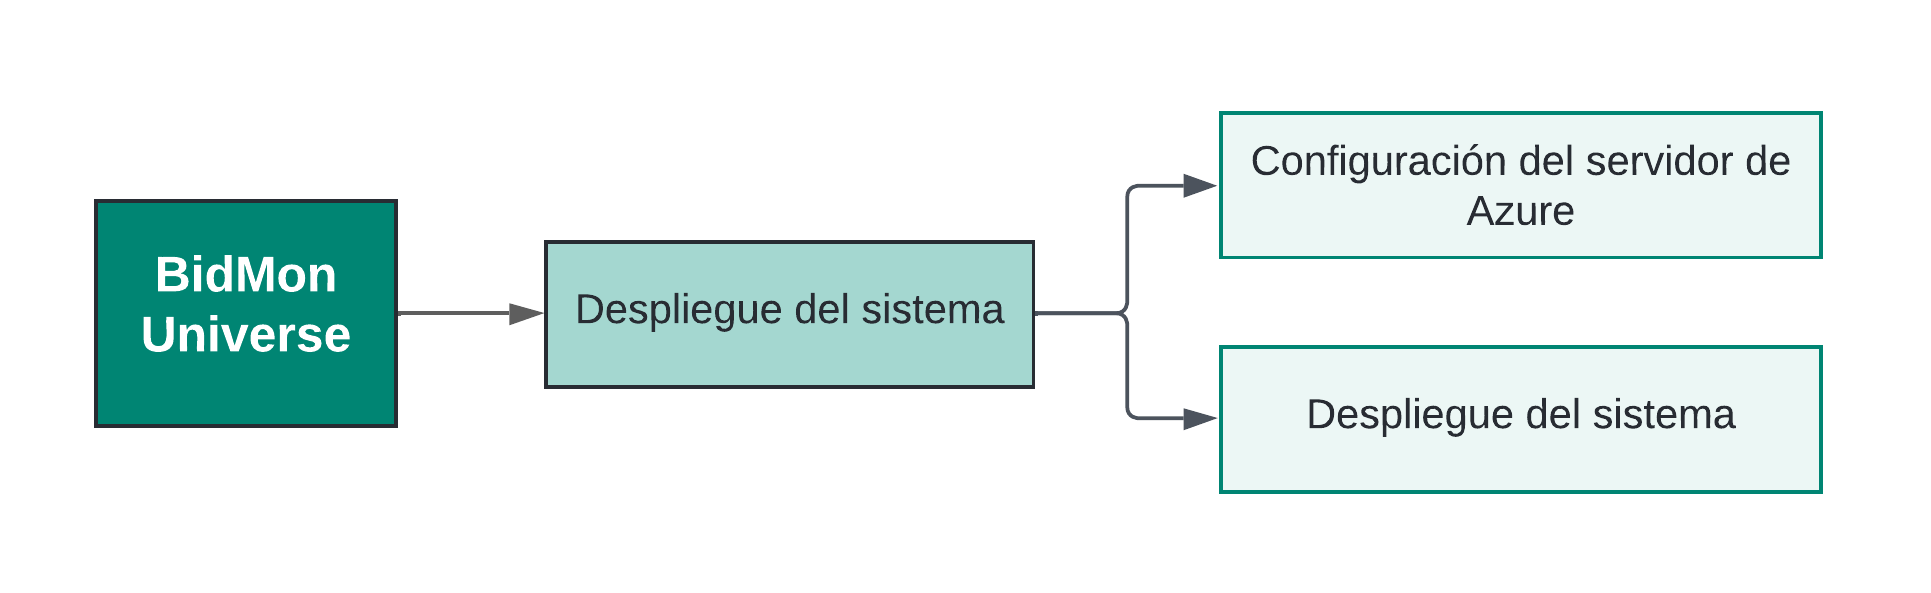
\includegraphics[width=0.9\linewidth]{figures/5-WBS/5_WBS-Despliegue2.png}
    \caption{WBS. Despliegue del sistema}
    \label{fig:5_WBS-Despliegue}
\end{figure}

\subsubsubsection{WBS. Documentación}
En la fase de documentación se realizan las tareas necesarias para la redacción de la memoria del proyecto, así como la preparación de la presentación del mismo.
\begin{figure}[H]
    \hypertarget{fig:5_WBS-Documentacion}{}
    \centering
    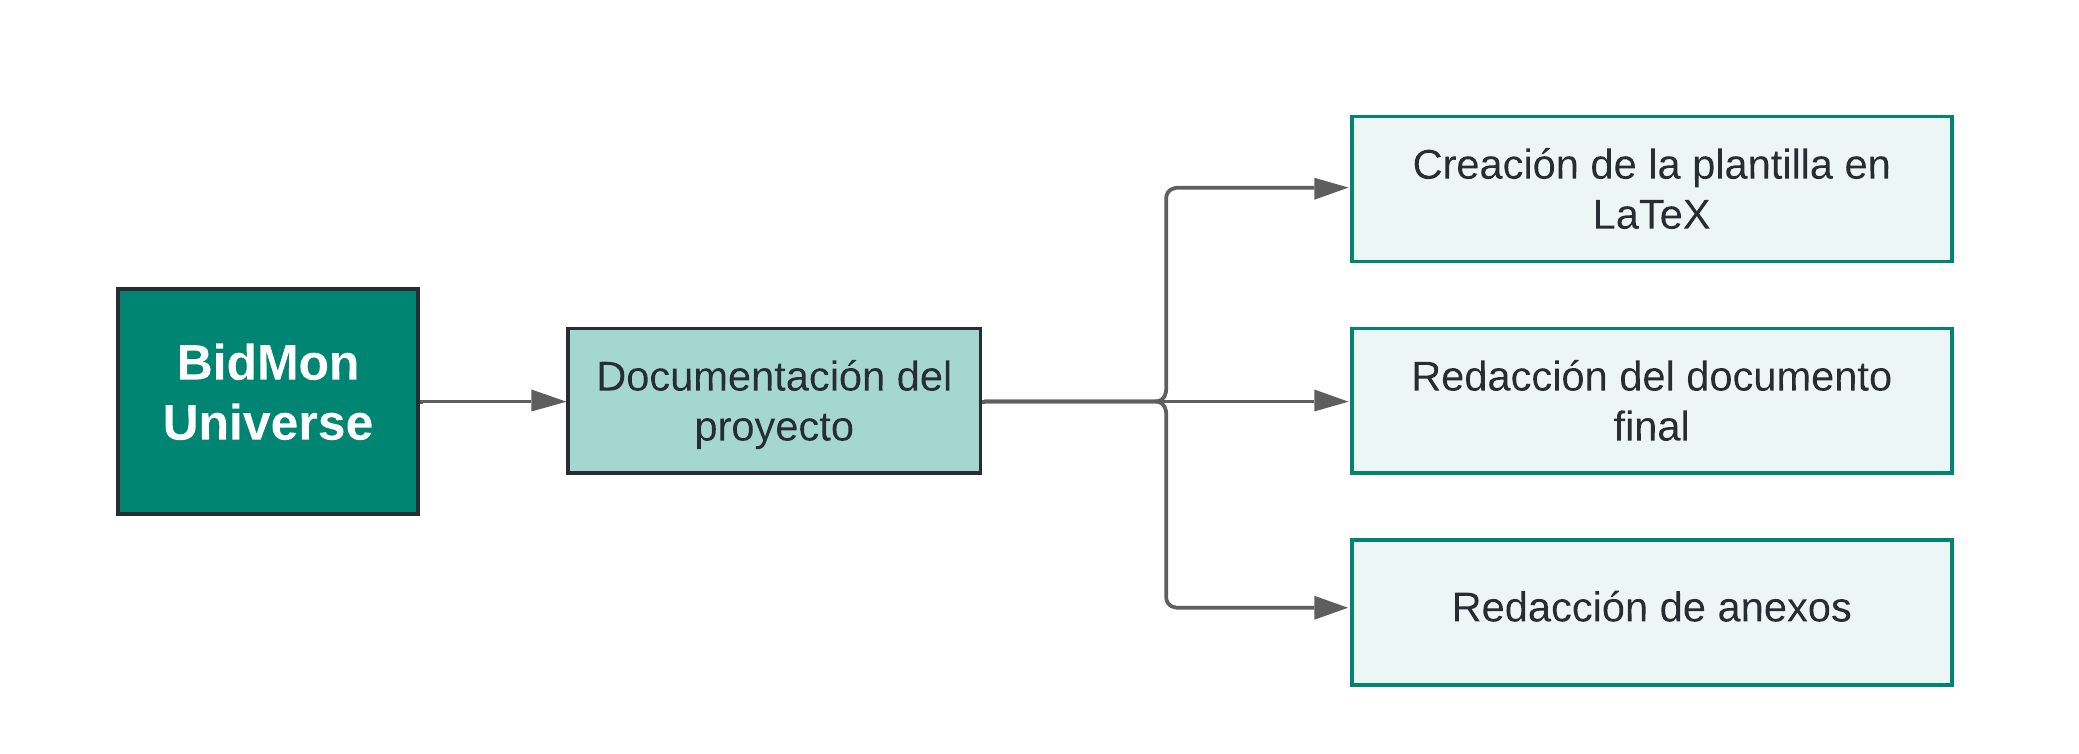
\includegraphics[width=0.9\linewidth]{figures/5-WBS/5_WBS-Documentacion.png}
    \caption{WBS. Documentación}
    \label{fig:5_WBS-Documentacion}
\end{figure}
